\documentclass[margin=5pt]{standalone}
% \usepackage[a4paper]{geometry}
\usepackage[utf8]{inputenc}
\usepackage{xifthen}
\usepackage{tikz}
% \usetikzlibrary{patterns}
\usetikzlibrary{math,calc}

% Setting background and foreground layers so we can draw some things over others
% https://tikz.dev/base-layers
\pgfdeclarelayer{background}
\pgfdeclarelayer{foreground}
\pgfsetlayers{background,main,foreground}

\title{Electoral College 2024 cartogram}
\author{Stuart Presnell}
\date{November 5th 2024}


\begin{document}

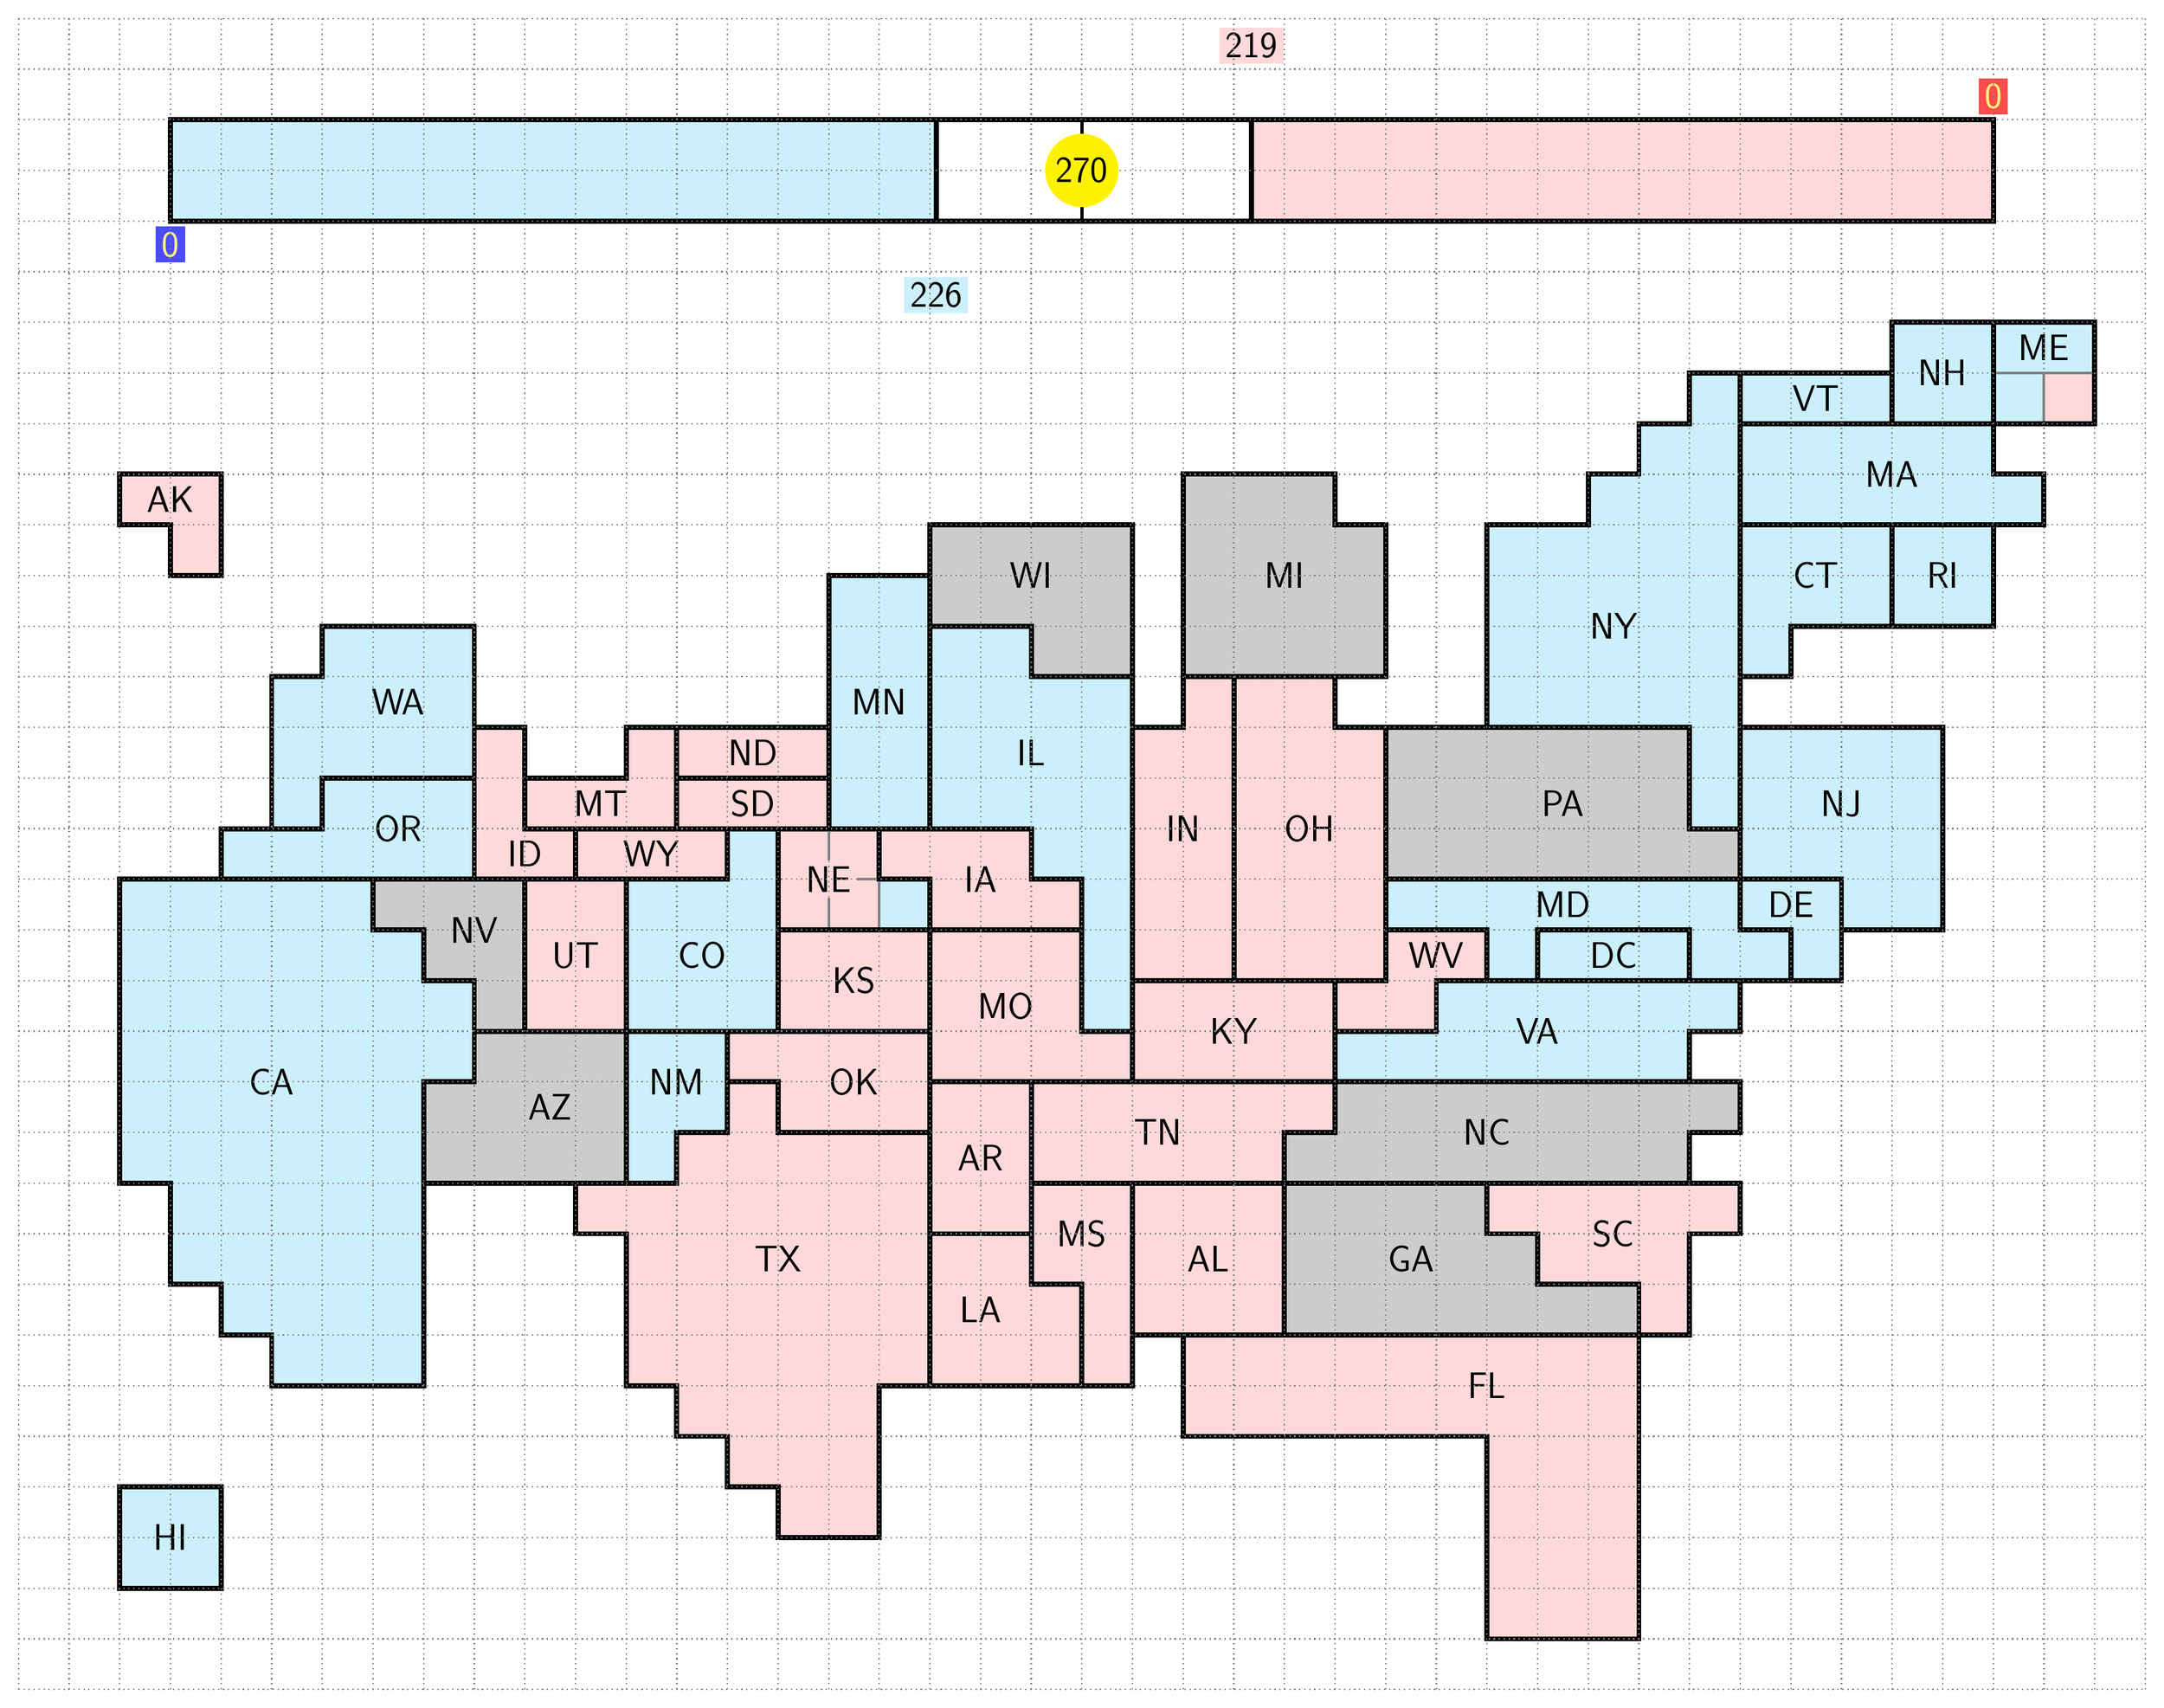
\begin{tikzpicture}\sffamily

%%%%%%%%%%%%%%%%%%%%%%%%%%%%%%%%%%%%%%%%%%%%%%%%%%

% This file defines the state styles HI, AK, etc. used in draw-states.tex
% This is where we record all the data about who has won each state
%   (or who is modelled/predicted to win each state)
%%!TEX root=main.tex

% In this file we record the status of each state as the results come in.
% Each state on the map has its own style that has been used to colour it; 
% 	here we define those state styles in terms of some pre-defined styles wait, wait, etc.

\tikzstyle{AK}=[wait]	%  3	Alaska
\tikzstyle{AL}=[wait]	%  9	Alabama
\tikzstyle{AR}=[wait]	%  6	Arkansas
\tikzstyle{AZ}=[wait]	% 11	Arizona
\tikzstyle{CA}=[wait]	% 54	California
\tikzstyle{CO}=[wait]	% 10	Colorado
\tikzstyle{CT}=[wait]	%  7	Connecticut
\tikzstyle{DC}=[wait]	%  3	District of Columbia*
\tikzstyle{DE}=[wait]	%  3	Delaware
\tikzstyle{FL}=[wait]	% 30	Florida
\tikzstyle{GA}=[wait]	% 16	Georgia
\tikzstyle{HI}=[wait]	%  4	Hawaii
\tikzstyle{IA}=[wait]	%  6	Iowa
\tikzstyle{ID}=[wait]	%  4	Idaho
\tikzstyle{IL}=[wait]	% 19	Illinois
\tikzstyle{IN}=[wait]	% 11	Indiana
\tikzstyle{KS}=[wait]	%  6	Kansas
\tikzstyle{KY}=[wait]	%  8	Kentucky
\tikzstyle{LA}=[wait]	%  8	Louisiana
\tikzstyle{MA}=[wait]	% 11	Massachusetts
\tikzstyle{MD}=[wait]	% 10	Maryland

%\tikzstyle{ME}=[wait]	% Maine**
\tikzstyle{M0}=[wait]	%  2	Maine popular vote winner
\tikzstyle{M1}=[wait]	%  1	Maine district 1
\tikzstyle{M2}=[wait]	%  1	Maine district 2

\tikzstyle{MI}=[wait]	% 15	Michigan
\tikzstyle{MN}=[wait]	% 10	Minnesota
\tikzstyle{MO}=[wait]	% 10	Missouri
\tikzstyle{MS}=[wait]	%  6	Mississippi
\tikzstyle{MT}=[wait]	%  4	Montana
\tikzstyle{NC}=[wait]	% 16	North Carolina
\tikzstyle{ND}=[wait]	%  3	North Dakota

%\tikzstyle{NE}=[wait]	% Nebraska**
\tikzstyle{N0}=[wait]	%  2	Nebraska popular vote winner
\tikzstyle{N1}=[wait]	%  1	Nebraska district 1
\tikzstyle{N2}=[wait]	%  1	Nebraska district 2
\tikzstyle{N3}=[wait]	%  1	Nebraska district 3

\tikzstyle{NH}=[wait]	%  4	New Hampshire
\tikzstyle{NJ}=[wait]	% 14	New Jersey
\tikzstyle{NM}=[wait]	%  5	New Mexico
\tikzstyle{NV}=[wait]	%  6	Nevada
\tikzstyle{NY}=[wait]	% 28	New York
\tikzstyle{OH}=[wait]	% 17	Ohio
\tikzstyle{OK}=[wait]	%  7	Oklahoma
\tikzstyle{OR}=[wait]	%  8	Oregon
\tikzstyle{PA}=[wait]	% 19	Pennsylvania
\tikzstyle{RI}=[wait]	%  4	Rhode Island
\tikzstyle{SC}=[wait]	%  9	South Carolina
\tikzstyle{SD}=[wait]	%  3	South Dakota
\tikzstyle{TN}=[wait]	% 11	Tennessee
\tikzstyle{TX}=[wait]	% 40	Texas
\tikzstyle{UT}=[wait]	%  6	Utah
\tikzstyle{VA}=[wait]	% 13	Virginia
\tikzstyle{VT}=[wait]	%  3	Vermont
\tikzstyle{WA}=[wait]	% 12	Washington
\tikzstyle{WI}=[wait]	% 10	Wisconsin
\tikzstyle{WV}=[wait]	%  4	West Virginia
\tikzstyle{WY}=[wait]	%  3	Wyoming



% How many Electoral College votes the above wins and expectations give each candidate:

\def\waitcount{0};
\def\Dwincount{0};
\def\waitcount{0};
\def\Rwincount{0};

%%!TEX root=main.tex

% In this file we record the status of each state as the results come in.
%  For each state, change the value in square brackets
%  The defined styles are:
%   Dfav: D candidate is favored to win — light blue
%   Rfav: R candidate is favored to win — light pink
%   Dwin: D candidate has won — dark blue
%   Rwin: R candidate has won — dark red
%   toss: The race is a tossup — light gray

\tikzstyle{AK}=[Rwin]	% Alaska
\tikzstyle{AL}=[Rwin]	% Alabama
\tikzstyle{AR}=[Rwin]	% Arkansas
\tikzstyle{AZ}=[Dwin]	% Arizona
\tikzstyle{CA}=[Dwin]	% California
\tikzstyle{CO}=[Dwin]	% Colorado
\tikzstyle{CT}=[Dwin]	% Connecticut
\tikzstyle{DC}=[Dwin]	% District of Columbia*
\tikzstyle{DE}=[Dwin]	% Delaware
\tikzstyle{FL}=[Rwin]	% Florida
\tikzstyle{GA}=[Dwin]	% Georgia
\tikzstyle{HI}=[Dwin]	% Hawaii
\tikzstyle{IA}=[Rwin]	% Iowa
\tikzstyle{ID}=[Rwin]	% Idaho
\tikzstyle{IL}=[Dwin]	% Illinois
\tikzstyle{IN}=[Rwin]	% Indiana
\tikzstyle{KS}=[Rwin]	% Kansas
\tikzstyle{KY}=[Rwin]	% Kentucky
\tikzstyle{LA}=[Rwin]	% Louisiana
\tikzstyle{MA}=[Dwin]	% Massachusetts
\tikzstyle{MD}=[Dwin]	% Maryland

%\tikzstyle{ME}=[wait]	% Maine**
\tikzstyle{M0}=[Dwin]	% Maine popular vote winner
\tikzstyle{M1}=[Dwin]	% Maine district 1
\tikzstyle{M2}=[Rwin]	% Maine district 2

\tikzstyle{MI}=[Dwin]	% Michigan
\tikzstyle{MN}=[Dwin]	% Minnesota
\tikzstyle{MO}=[Rwin]	% Missouri
\tikzstyle{MS}=[Rwin]	% Mississippi
\tikzstyle{MT}=[Rwin]	% Montana
\tikzstyle{NC}=[Rwin]	% North Carolina
\tikzstyle{ND}=[Rwin]	% North Dakota

%\tikzstyle{NE}=[wait]	% Nebraska**
\tikzstyle{N0}=[Rwin]	% Nebraska popular vote winner
\tikzstyle{N1}=[Rwin]	% Nebraska district 1
\tikzstyle{N2}=[Rwin]	% Nebraska district 2
\tikzstyle{N3}=[Dwin]	% Nebraska district 3

\tikzstyle{NH}=[Dwin]	% New Hampshire
\tikzstyle{NJ}=[Dwin]	% New Jersey
\tikzstyle{NM}=[Dwin]	% New Mexico
\tikzstyle{NV}=[Dwin]	% Nevada
\tikzstyle{NY}=[Dwin]	% New York
\tikzstyle{OH}=[Rwin]	% Ohio
\tikzstyle{OK}=[Rwin]	% Oklahoma
\tikzstyle{OR}=[Dwin]	% Oregon
\tikzstyle{PA}=[Dwin]	% Pennsylvania
\tikzstyle{RI}=[Dwin]	% Rhode Island
\tikzstyle{SC}=[Rwin]	% South Carolina
\tikzstyle{SD}=[Rwin]	% South Dakota
\tikzstyle{TN}=[Rwin]	% Tennessee
\tikzstyle{TX}=[Rwin]	% Texas
\tikzstyle{UT}=[Rwin]	% Utah
\tikzstyle{VA}=[Dwin]	% Virginia
\tikzstyle{VT}=[Dwin]	% Vermont
\tikzstyle{WA}=[Dwin]	% Washington
\tikzstyle{WI}=[Dwin]	% Wisconsin
\tikzstyle{WV}=[Rwin]	% West Virginia
\tikzstyle{WY}=[Rwin]	% Wyoming


% How many Electoral College votes the above wins and expectations give each candidate:

\def\Dfavcount{0};
\def\Dwincount{306};
\def\Rfavcount{0};
\def\Rwincount{232};

%%!TEX root=main.tex

% In this file we record the status of each state as the results come in.
% Each state on the map has its own style that has been used to colour it; 
% 	here we define those state styles in terms of some pre-defined styles Dfav, Rfav, etc.

\tikzstyle{AK}=[Rfav]	%  3	Alaska
\tikzstyle{AL}=[Rfav]	%  9	Alabama
\tikzstyle{AR}=[Rfav]	%  6	Arkansas
\tikzstyle{AZ}=[toss]	% 11	Arizona
\tikzstyle{CA}=[Dfav]	% 54	California
\tikzstyle{CO}=[Dfav]	% 10	Colorado
\tikzstyle{CT}=[Dfav]	%  7	Connecticut
\tikzstyle{DC}=[Dfav]	%  3	District of Columbia*
\tikzstyle{DE}=[Dfav]	%  3	Delaware
\tikzstyle{FL}=[Rfav]	% 30	Florida
\tikzstyle{GA}=[toss]	% 16	Georgia
\tikzstyle{HI}=[Dfav]	%  4	Hawaii
\tikzstyle{IA}=[Rfav]	%  6	Iowa
\tikzstyle{ID}=[Rfav]	%  4	Idaho
\tikzstyle{IL}=[Dfav]	% 19	Illinois
\tikzstyle{IN}=[Rfav]	% 11	Indiana
\tikzstyle{KS}=[Rfav]	%  6	Kansas
\tikzstyle{KY}=[Rfav]	%  8	Kentucky
\tikzstyle{LA}=[Rfav]	%  8	Louisiana
\tikzstyle{MA}=[Dfav]	% 11	Massachusetts
\tikzstyle{MD}=[Dfav]	% 10	Maryland

%\tikzstyle{ME}=[Dfav]	% Maine**
\tikzstyle{M0}=[Dfav]	%  2	Maine popular vote winner
\tikzstyle{M1}=[Dfav]	%  1	Maine district 1
\tikzstyle{M2}=[Rfav]	%  1	Maine district 2

\tikzstyle{MI}=[toss]	% 15	Michigan
\tikzstyle{MN}=[Dfav]	% 10	Minnesota
\tikzstyle{MO}=[Rfav]	% 10	Missouri
\tikzstyle{MS}=[Rfav]	%  6	Mississippi
\tikzstyle{MT}=[Rfav]	%  4	Montana
\tikzstyle{NC}=[toss]	% 16	North Carolina
\tikzstyle{ND}=[Rfav]	%  3	North Dakota

%\tikzstyle{NE}=[Rfav]	% Nebraska**
\tikzstyle{N0}=[Rfav]	%  2	Nebraska popular vote winner
\tikzstyle{N1}=[Rfav]	%  1	Nebraska district 1
\tikzstyle{N2}=[Rfav]	%  1	Nebraska district 2
\tikzstyle{N3}=[Dfav]	%  1	Nebraska district 3

\tikzstyle{NH}=[Dfav]	%  4	New Hampshire
\tikzstyle{NJ}=[Dfav]	% 14	New Jersey
\tikzstyle{NM}=[Dfav]	%  5	New Mexico
\tikzstyle{NV}=[toss]	%  6	Nevada
\tikzstyle{NY}=[Dfav]	% 28	New York
\tikzstyle{OH}=[Rfav]	% 17	Ohio
\tikzstyle{OK}=[Rfav]	%  7	Oklahoma
\tikzstyle{OR}=[Dfav]	%  8	Oregon
\tikzstyle{PA}=[toss]	% 19	Pennsylvania
\tikzstyle{RI}=[Dfav]	%  4	Rhode Island
\tikzstyle{SC}=[Rfav]	%  9	South Carolina
\tikzstyle{SD}=[Rfav]	%  3	South Dakota
\tikzstyle{TN}=[Rfav]	% 11	Tennessee
\tikzstyle{TX}=[Rfav]	% 40	Texas
\tikzstyle{UT}=[Rfav]	%  6	Utah
\tikzstyle{VA}=[Dfav]	% 13	Virginia
\tikzstyle{VT}=[Dfav]	%  3	Vermont
\tikzstyle{WA}=[Dfav]	% 12	Washington
\tikzstyle{WI}=[toss]	% 10	Wisconsin
\tikzstyle{WV}=[Rfav]	%  4	West Virginia
\tikzstyle{WY}=[Rfav]	%  3	Wyoming



% How many Electoral College votes the above wins and expectations give each candidate:

\def\Dfavcount{226};
\def\Dwincount{0};
\def\Rfavcount{219};
\def\Rwincount{0};

%!TEX root=main.tex

% In this file we record the status of each state as the results come in.
%  For each state, change the value in square brackets
%  The defined styles are:
%   Dfav: D candidate is favored to win — light blue
%   Rfav: R candidate is favored to win — light pink
%   Dwin: D candidate has won — dark blue
%   Rwin: R candidate has won — dark red
%   toss: The race is a tossup — light gray

\tikzstyle{AK}=[Rfav]	%  3	Alaska
\tikzstyle{AL}=[Rfav]	%  9	Alabama
\tikzstyle{AR}=[Rfav]	%  6	Arkansas
\tikzstyle{AZ}=[toss]	% 11	Arizona
\tikzstyle{CA}=[Dfav]	% 54	California
\tikzstyle{CO}=[Dfav]	% 10	Colorado
\tikzstyle{CT}=[Dfav]	%  7	Connecticut
\tikzstyle{DC}=[Dfav]	%  3	District of Columbia*
\tikzstyle{DE}=[Dfav]	%  3	Delaware
\tikzstyle{FL}=[Rfav]	% 30	Florida
\tikzstyle{GA}=[toss]	% 16	Georgia
\tikzstyle{HI}=[Dfav]	%  4	Hawaii
\tikzstyle{IA}=[Rfav]	%  6	Iowa
\tikzstyle{ID}=[Rfav]	%  4	Idaho
\tikzstyle{IL}=[Dfav]	% 19	Illinois
\tikzstyle{IN}=[Rfav]	% 11	Indiana
\tikzstyle{KS}=[Rfav]	%  6	Kansas
\tikzstyle{KY}=[Rfav]	%  8	Kentucky
\tikzstyle{LA}=[Rfav]	%  8	Louisiana
\tikzstyle{MA}=[Dfav]	% 11	Massachusetts
\tikzstyle{MD}=[Dfav]	% 10	Maryland

%\tikzstyle{ME}=[Dfav]	% Maine**
\tikzstyle{M0}=[Dfav]	%  2	Maine popular vote winner
\tikzstyle{M1}=[Dfav]	%  1	Maine district 1
\tikzstyle{M2}=[Rfav]	%  1	Maine district 2

\tikzstyle{MI}=[toss]	% 15	Michigan
\tikzstyle{MN}=[Dfav]	% 10	Minnesota
\tikzstyle{MO}=[Rfav]	% 10	Missouri
\tikzstyle{MS}=[Rfav]	%  6	Mississippi
\tikzstyle{MT}=[Rfav]	%  4	Montana
\tikzstyle{NC}=[toss]	% 16	North Carolina
\tikzstyle{ND}=[Rfav]	%  3	North Dakota

%\tikzstyle{NE}=[Rfav]	% Nebraska**
\tikzstyle{N0}=[Rfav]	%  2	Nebraska popular vote winner
\tikzstyle{N1}=[Rfav]	%  1	Nebraska district 1
\tikzstyle{N2}=[Rfav]	%  1	Nebraska district 2
\tikzstyle{N3}=[Dfav]	%  1	Nebraska district 3

\tikzstyle{NH}=[Dfav]	%  4	New Hampshire
\tikzstyle{NJ}=[Dfav]	% 14	New Jersey
\tikzstyle{NM}=[Dfav]	%  5	New Mexico
\tikzstyle{NV}=[toss]	%  6	Nevada
\tikzstyle{NY}=[Dfav]	% 28	New York
\tikzstyle{OH}=[Rfav]	% 17	Ohio
\tikzstyle{OK}=[Rfav]	%  7	Oklahoma
\tikzstyle{OR}=[Dfav]	%  8	Oregon
\tikzstyle{PA}=[toss]	% 19	Pennsylvania
\tikzstyle{RI}=[Dfav]	%  4	Rhode Island
\tikzstyle{SC}=[Rfav]	%  9	South Carolina
\tikzstyle{SD}=[Rfav]	%  3	South Dakota
\tikzstyle{TN}=[Rfav]	% 11	Tennessee
\tikzstyle{TX}=[Rfav]	% 40	Texas
\tikzstyle{UT}=[Rfav]	%  6	Utah
\tikzstyle{VA}=[Dfav]	% 13	Virginia
\tikzstyle{VT}=[Dfav]	%  3	Vermont
\tikzstyle{WA}=[Dfav]	% 12	Washington
\tikzstyle{WI}=[toss]	% 10	Wisconsin
\tikzstyle{WV}=[Rfav]	%  4	West Virginia
\tikzstyle{WY}=[Rfav]	%  3	Wyoming



% How many Electoral College votes the above wins and expectations give each candidate:
% Unfortunately I haven't figured out how to update this automatically from the above data,
%  so these numbers must be edited manually as results come in

\def\Dfavcount{226};
\def\Rfavcount{219};

\def\Dwincount{0};
\def\Rwincount{0};


%%%%%%%%%%%%%%%%%%%%%%%%%%%%%%%%%%%%%%%%%%%%%%%%%%


% Parameters setting the size of the diagram
\def\xmin{0};
\def\xmax{42};
\def\ymin{-1};
\def\ymax{32};

% Define some named colouring styles
\tikzstyle{wait}=[fill=white,   font=\huge, text=black]
\tikzstyle{toss}=[fill=gray!40, font=\huge, text=black]
\tikzstyle{Dwin}=[fill=blue!70, font=\huge, text=yellow!50!white]
\tikzstyle{Rwin}=[fill=red!70,  font=\huge, text=yellow!50!white]
\tikzstyle{Dfav}=[fill=cyan!20, font=\huge, text=black]
\tikzstyle{Rfav}=[fill=pink!60, font=\huge, text=black]

\tikzstyle{state}=[line width=1mm]
\tikzstyle{district}=[gray, line width=0.5mm]
% \tikzstyle{lake}=[fill=white]
\tikzstyle{label}=[font=\huge, text=black]


% Dotted grid lines
\begin{pgfonlayer}{foreground}
\draw[step=1cm,gray,dotted,thick] (\xmin,\ymin) grid (\xmax,\ymax);
\end{pgfonlayer}


%%%%%%%%%%%%%%%%%%%%%%%%%
%%%%%%%%%%%%%%%%%%%%%%%%%

% Import commands for drawing the Electoral College progress bar
%!TEX root=main.tex

% Drawing the Electoral College progress bar

%% Example usage:
%\leftbar{300}{Dfav};
%\leftbar{273}{Dwin};
%\rightbar{100}{Rfav};
%\rightbar{50}{Rwin};
%% These are on the main layer, so between the grey background and the foreground labels
%% Remember to draw each of the (longer) Xfav bars before the (shorter) Xwin bars


% Style for text labels
\tikzstyle{bartext}=[black, font=\huge]

% Parameters setting the left, right, bottom and top of the bar
%  The bar is 36 units wide, so each step corresponds to 15 EC votes
\def\barL{3}
\def\barR{39}
\def\barB{28}
\def\barT{30}

% Calculate the horizontal midpoint of the bar
\pgfmathparse{(\barL + \barR)/2};
\edef\barM{\pgfmathresult}

% Calculate the vertical midpoint of the bar
\pgfmathparse{(\barT + \barB)/2};
\edef\barC{\pgfmathresult}

% Draw the EC progress bar rectangle on the background layer;
%  This ensures that subsequent bars drawn on main are over this background
\begin{pgfonlayer}{background}
	\draw[wait, state] (\barL,\barB) rectangle (\barR,\barT);
\end{pgfonlayer}

% Draw and label the midpoint of the bar on the foreground layer
%  This ensures that the line is still visible when we draw bars on main
\begin{pgfonlayer}{foreground}
	\draw[ultra thick, black] (\barM,\barT) -- (\barM,\barB);
	\node[circle, black, fill=yellow, font=\huge] at (\barM,\barC) {270};
\end{pgfonlayer}



% Draw a rectangle from the left of the EC bar of length (#1/538) the bar
% Styled as #2, with label at position #3
\newcommand{\leftbar}[3]{
	\pgfmathparse{\barL + ((\barR - \barL)*(#1/538))};	
	\edef\barX{\pgfmathresult}
	
	\draw[state, #2] (\barL,\barT) rectangle (\barX,\barB);
	\node[bartext, below=#3mm, #2] at (\barX,\barB) {#1};
}


% Draw a rectangle from the right of the EC bar of length (#1/538) the bar
% Styled as #2, with label at position #3
\newcommand{\rightbar}[3]{
	\pgfmathparse{\barL + ((\barR - \barL)*(1 - #1/538))};	
	\edef\barX{\pgfmathresult}
	
	\draw[state, #2] (\barR,\barT) rectangle (\barX,\barB);
	\node[bartext, above=#3mm, #2] at (\barX,\barT) {#1};
}


% Now bundle these into commands for the 4 bars we want to draw

\newcommand{\Dfavbar}[1]{
	\leftbar{#1}{Dfav}{11};
}

\newcommand{\Dwinbar}[1]{
	\leftbar{#1}{Dwin}{1};
}

\newcommand{\Rfavbar}[1]{
	\rightbar{#1}{Rfav}{11};
}

\newcommand{\Rwinbar}[1]{
	\rightbar{#1}{Rwin}{1};
}



% Now draw the actual bars
% Remember to draw each of the (longer) Xfav bars before the (shorter) Xwin bars
\Dfavbar{\Dfavcount};
\Dwinbar{\Dwincount};
\Rfavbar{\Rfavcount};
\Rwinbar{\Rwincount};

%%%%%%%%%%%%%%%%%%%%%%%%%
%%%%%%%%%%%%%%%%%%%%%%%%%

% Draw the state boundaries and colour them by their state styles HI, AK, etc.
% These state styles are defined in the data file input at the top e.g. 2020-results.tex
%!TEX root=main.tex


% Drawing commands to draw straight lines in cardinal directions Up, Down, East, West
\newcommand{\U}[1]{++(0,#1)}
\newcommand{\D}[1]{++(0,-#1)}
\newcommand{\E}[1]{++(#1,0)}
\newcommand{\W}[1]{++(-#1,0)}


% Draw the state boundaries and colour them by their state styles HI, AK, etc.

% HI
\draw[state, HI] (2,1) rectangle ++(2,2);
\node[HI] at (3,2) (HI) {HI};

% AK
\draw[state, AK] (2,23) -- \D{1} -- \E{1} -- \D{1} -- \E{1} -- \U{2} -- cycle;
\node[AK] at (3,22.5) (AK) {AK};


% CA
\draw[state, CA] 
(2,15) -- \D{6} -- \E{1} -- 
\D{2} -- 
\E{1} -- \D{1} -- 
\E{1} -- \D{1} -- 
\E{3} -- \U{6} -- \E{1} -- \U{2} 
-- \W{1} -- \U{1} -- \W{1} -- \U{1} -- cycle;
\node[CA] at (5,11) (CA) {CA};


% OR
\draw[state, OR] 
(5,15) -- \E{4} -- \U{2} -- 
\W{3} -- \D{1} -- \W{2} -- \D{1} -- cycle;
\node[OR] at (7.5,16) (OR) {OR};


% WA
\draw[state, WA] (5,16) -- \E{1} -- \U{1} -- \E{3} -- \U{3} -- 
\W{3} -- \D{1} -- \W{1} -- cycle;
\node[WA] at (7.5,18.5) (WA) {WA};


% AZ
\draw[state, AZ] (8,9) -- \E{4} -- \U{3} -- \W{3} --
\D{1} -- \W{1} -- cycle;
\node[AZ] at (10.5,10.5) (AZ) {AZ};


% NV
\draw[state, NV] (7,15) -- 
\D{1} -- \E{1} -- 
\D{1} -- \E{1} -- 
\D{1} -- \E{1} -- \U{3} -- cycle;
\node[NV] at (9,14) (NV) {NV};

% ID
\draw[state, ID] (9,15) -- \E{2} -- 
\U{1} -- \W{1} --
\U{2} -- \W{1} -- cycle;
\node[ID] at (10,15.5) (ID) {ID};


% UT
\draw[state, UT] (10,12) rectangle ++(2,3);
\node[UT] at (11,13.5) (UT) {UT};

% CO
\draw[state, CO] 
(12,12) --
\E{3} -- 
\U{4} -- \W{1} -- \D{1} -- \W{2} --
cycle;
\node[CO] at (13.5,13.5) (CO) {CO};

% NM
\draw[state, NM] (12,12) --
\D{3} -- \E{1} -- 
\U{1} -- \E{1} -- 
\U{2} -- \W{2} -- cycle;
\node[NM] at (13,11) (NM) {NM};

% MT
\draw[state, MT] 
(10,16) -- 
\E{3} -- 
\U{2} -- 
\W{1} -- 
\D{1} -- 
\W{2} -- 
cycle;
\node[MT] at (11.5,16.5) (MT) {MT};

% WY
\draw[state, WY] (11,15) rectangle ++(3,1);
\node[WY] at (12.5,15.5) (WY) {WY};

% SD
\draw[state, SD] (13,16) rectangle ++(3,1);
\node[SD] at (14.5,16.5) (SD) {SD};

% ND
\draw[state, ND] (13,17) rectangle ++(3,1);
\node[ND] at (14.5,17.5) (ND) {ND};

% KS
\draw[state, KS] (15,12) rectangle ++(3,2);
\node[KS] at (16.5,13) (KS) {KS};

% OK
\draw[state, OK] (14,11) -- 
\E{1} -- \D{1} --
\E{3} -- \U{2} -- \W{4} -- cycle;
\node[OK] at (16.5,11) (OK) {OK};

% TX
\draw[state, TX] (11,9) -- 
\D{1} -- \E{1} -- 
\D{3} -- \E{1} -- 
\D{1} -- \E{1} -- 
\D{1} -- \E{1} -- 
\D{1} -- \E{2} -- 
\U{2} -- %\E{1} -- 
\U{1} -- \E{1} -- 
\U{5} -- \W{3} -- 
\U{1} -- \W{1} -- 
\D{1} -- \W{1} -- 
\D{1} -- 
cycle;
\node[TX] at (15,7.5) (TX) {TX};


% MN
\draw[state, MN] (16,16) rectangle ++(2,5);
\node[MN] at (17,18.5) (MN) {MN};


% MO
\draw[state, MO] (18,11)-- 
\E{4} -- 
\U{1} -- \W{1} --
\U{2} -- \W{3} -- cycle;
\node[MO] at (19.5,12.5) (MO) {MO};

% AR
\draw[state, AR] (18,8) rectangle ++(2,3);
\node[AR] at (19,9.5) (AR) {AR};

% LA
\draw[state, LA] (18,5)-- 
\E{3} -- 
\U{2} -- \W{1} --
\U{1} -- \W{2} -- cycle;
\node[LA] at (19,6.5) (LA) {LA};


% WI
\draw[state, WI] (18,20) -- 
\E{2} -- \D{1} --
\E{2} -- \U{3} -- \W{4} -- cycle;
\node[WI] at (20,21) (WI) {WI};


% IA
\draw[state, IA] (18,14) -- 
\E{3} -- \U{1} -- 
\W{1} -- \U{1} -- 
\W{3} -- 
\D{1} -- 
\E{1} -- 
cycle;
\node[IA] at (19,15) (IA) {IA};

% IL
\draw[state, IL] (18,20) -- 
\D{4} -- \E{2} -- \D{1} -- \E{1} -- \D{3} -- 
\E{1} -- \U{7} -- \W{2} -- \U{1} -- 
cycle;
\node[IL] at (20,17.5) (IL) {IL};

% IN
\draw[state, IN] (22,13) -- 
\E{2} -- \U{6} -- 
\W{1} -- \D{1} -- \W{1} -- cycle;
\node[IN] at (23,16) (IN) {IN};

% KY
\draw[state, KY] (22,11) rectangle ++(4,2);
\node[KY] at (24,12) (KY) {KY};

% TN
\draw[state, TN] (20,11) --
\D{2} -- \E{5} -- 
\U{1} -- \E{1} -- 
\U{1} -- \W{6} -- 
cycle;
\node[TN] at (22.5,10) (TN) {TN};

% MS
\draw[state, MS] (20,7) -- 
\E{1} -- \D{2} --
\E{1} -- \U{4} -- \W{2} -- cycle;
\node[MS] at (21,8) (MS) {MS};

% AL
\draw[state, AL] (22,6) rectangle ++(3,3);
\node[AL] at (23.5,7.5) (AL) {AL};

% GA
\draw[state, GA] (25,6) -- 
\E{7} -- 
\U{1} -- \W{2} --
\U{1} -- \W{1} --
\U{1} -- \W{4} -- cycle;
\node[GA] at (27.5,7.5) (GA) {GA};

% SC
\draw[state, SC] (29,9) -- 
\D{1} -- \E{1} -- 
\D{1} -- \E{2} -- 
\D{1} -- \E{1} -- 
\U{2} -- 
\E{1} -- \U{1} -- 
cycle;
\node[SC] at (31.5,8) (SC) {SC};

% FL
\draw[state, FL] (23,6) -- 
\D{2} -- \E{6} -- 
\D{4} -- \E{3} -- \U{6} -- cycle;
\node[FL] at (29,5) (FL) {FL};


% NC
\draw[state, NC] (25,9) -- 
\E{8} -- 
\U{1} -- \E{1} -- \U{1} -- \W{8} -- 
\D{1} -- \W{1} -- cycle;
\node[NC] at (29,10) (NC) {NC};

% VA
\draw[state, VA] (26,11) -- 
\E{7} -- \U{1} -- 
\E{1} -- \U{1} -- 
\W{6} -- \D{1} -- \W{2} --
cycle;
\node[VA] at (30,12) (VA) {VA};



% DC
\draw[state, DC] (30,13) rectangle ++(3,1);
\node[DC] at (31.5,13.5) (DC) {DC};

% MD
\draw[state, MD] (27,15) -- 
\D{1} -- \E{2} -- 
\D{1} -- \E{1} -- 
\U{1} -- \E{3} -- 
\D{1} -- \E{2} -- 
\U{1} -- \W{1} -- 
\U{1} -- \W{7} -- 
cycle;
\node[MD] at (30.5,14.5) (MD) {MD};

% DE
\draw[state, DE] (34,14) -- 
\E{1} -- \D{1} --
\E{1} -- \U{2} -- \W{2} -- cycle;
\node[DE] at (35,14.5) (DE) {DE};

% NJ
\draw[state, NJ] (34,15) -- 
\E{2} -- \D{1} --
\E{2} -- \U{4} -- \W{4} -- cycle;
\node[NJ] at (36,16.5) (NJ) {NJ};


% NY
\draw[state, NY] (29,18) -- 
\E{4} -- 
%\D{1} -- \E{1} -- \U{8} -- 
\D{2} -- \E{1} -- \U{9} -- \W{1} -- \D{1} -- 
\W{1} -- \D{1} -- \W{1} -- \D{1} -- 
\W{2} -- 
cycle;
\node[NY] at (31.5,20) (NY) {NY};

% VT
\draw[state, VT] (34,24) rectangle ++(3,1);
\node[VT] at (35.5,24.5) (VT) {VT};

% NH
\draw[state, NH] (37,24) rectangle ++(2,2);
\node[NH] at (38,25) (NH) {NH};

% MA
\draw[state, MA] (34,22)-- 
\E{6} -- 
\U{1} -- \W{1} --
\U{1} -- \W{5} -- cycle;
\node[MA] at (37,23) (MA) {MA};

% CT
\draw[state, CT] (34,22) --
\D{3} -- \E{1} -- 
\U{1} -- \E{2} -- \U{2} -- \W{3} -- 
cycle;
\node[CT] at (35.5,21) (CT) {CT};

% RI
\draw[state, RI] (37,20) rectangle ++(2,2);
\node[RI] at (38,21) (RI) {RI};


% WV
\draw[state, WV] (26,12) --
\E{2} -- \U{1} -- \E{1} -- \U{1} -- 
%\W{3} -- 
\W{2} -- 
\D{1} -- 
\W{1} -- 
cycle;
\node[WV] at (28,13.5) (WV) {WV};


% OH
\draw[state, OH] (24,13) -- 
\E{3} -- \U{5} -- 
\W{1} -- \U{1} -- \W{2} -- cycle;
\node[OH] at (25.5,16) (OH) {OH};

% MI
\draw[state, MI] (23,19) -- 
\E{4} -- \U{3} -- 
\W{1} -- \U{1} -- 
\W{3} -- cycle;
\node[MI] at (25,21) (MI) {MI};

% PA
\draw[state, PA] (27,15)-- 
\E{7} -- 
\U{1} -- \W{1} -- \U{2} -- 
\W{6} -- cycle;
\node[PA] at (30.5,16.5) (PA) {PA};

%%%%%%%%%%%%%%%%%%%%%%%%%%%%%%%%%%%%%%%%%%%%%%%%%%

% NEBRASKA and its districts
%	In the 2024 election, 
%	Nebraska allocates 2 electoral votes to the state popular vote winner, 
%	and then one electoral vote to the winner in each of 3 districts

% NE popular vote winner
\draw[district, N0] (15,16) -- 
\D{2} --
\E{1} -- \U{2} -- 
cycle;

% NE district 1
\draw[district, N1] (16,16) -- 
\D{1} --
\E{1} -- \U{1} -- 
cycle;

% NE district 2
\draw[district, N2] (16,15) -- 
\D{1} --
\E{1} -- \U{1} -- 
cycle;

% NE district 3
\draw[district, N3] (17,15) -- 
\D{1} --
\E{1} -- \U{1} -- 
cycle;

% NE - drawing the state boundary
\draw[state] (15,16) -- 
\D{2} --
\E{3} -- \U{1} -- \W{1} -- \U{1} -- 
cycle;
\node[N0] at (16,15) (NE) {NE};  

%%%%%%%%%%%%%%%%%%%%%%%%%%%%%%%%%%%%%%%%%%%%%%%%%%

% MAINE and its districts
%	In the 2024 election, 
%	Maine allocates 2 electoral votes to the state popular vote winner, 
%	and then one electoral vote to the winner in each of 2 districts

% ME popular vote winner
\draw[district, M0] (39,25) rectangle ++(2,1);

%% ME district 1
\draw[district, M1] (39,24) rectangle ++(1,1);

% ME district 2
\draw[district, M2] (40,24) rectangle ++(1,1);

% ME - drawing the state boundary
\draw[state] (39,24) rectangle ++(2,2);
\node[M0] at (40,25.5) (ME) {ME};

%%%%%%%%%%%%%%%%%%%%%%%%%%%%%%%%%%%%%%%%%%%%%%%%%%



% Optionally, a couple of lakes; 
% but need to choose colouring for these that doesn't clash with blue for Dem

% % Lake Michigan
% \draw[state, lake] (22,18) rectangle ++(1,4);

% % Lake Erie / Lake Ontario
%\draw[state, lake] 
%(26,18) --
%\E{3} -- \U{4} -- \W{2} -- \D{3} -- \W{1} -- cycle;



%%%%%%%%%%%%%%%%%%%%%%%%%
%%%%%%%%%%%%%%%%%%%%%%%%%

% Optionally, an info box in the lower right corner
%\draw[ultra thick] (41,0) rectangle ++(-5,10);

%% Experimenting with trying to calculate EC totals automatically
%\ifthenelse
% {\equal{1}{1}}
%	{\draw[fill=green] (39,5) circle (1cm) {};}
%	{\draw[fill=red] (39,5) circle (1cm) {};}
%\foreach \s[
%	remember=\j as \j (initially 0), 
%	evaluate=\j using \j+3
%] in {HI, AK} {}; % Don't draw anything on each loop, just using the end result.
%\node[black, font=\huge] at (40,1) {$\j$};





\end{tikzpicture}

\end{document}










